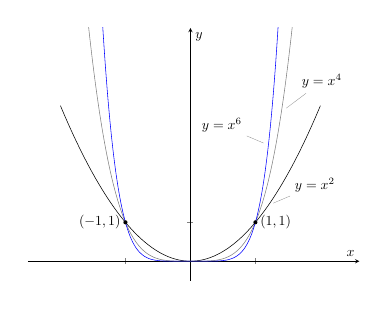
\begin{tikzpicture}[scale=0.5]
\begin{axis}[
  %title = {$f(x)=x^n$, $n=2k$, $k \in \mathrm{Z}_{+}$},
 axis lines=middle,
 ticklabel style={fill=white},
 xmin=-2.5,xmax=2.6,
 ymin=-0.5,ymax=6,
 xlabel=$x$,ylabel=$y$,
 domain=-2:2,
 samples=100,
 smooth,
 xtick={-1,0,1},ytick={1},
 yticklabels={,,},   xticklabels={,,},
 width=10cm, height=8cm]
\coordinate  (x2) at (1,1);
\coordinate (x1) at (-1,1);

\addplot[black] { x^2};
\addplot[gray] {x^4};
\addplot[blue] {x^6};
\fill[black] (x1) circle (1.5pt);
\fill[black] (x2) circle (1.5pt);

\node[pin= 20:{$y=x^2$}] at (axis cs:1.2,{(1.2)^2}) {};
\node[pin= 50:{$y=x^4$}] at (axis cs:1.4,{(1.4)^4}) {};
\node[pin= 160:{$y=x^6$}] at (axis cs:1.2,{(1.2)^6}) {};
\node[right] at (x2) {$(1,1)$};
\node[left] at (x1) {$(-1,1)$};
\end{axis}
\end{tikzpicture}














